\section{\label{results}Results}



\begin{figure}
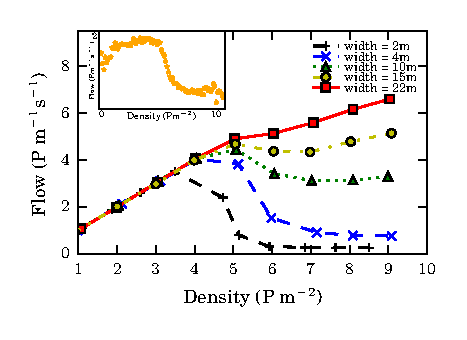
\includegraphics[width=\columnwidth]
{plots/flow-density_vd1_multiple_widths.eps}
\caption{\label{fig:1} Flow as a function of the density for different widths. Inittialy, 
pedestrians were random distributed along the corridor. The measurements were taken in the middle
of the corridor once the system reached the stationary state. The lenght of the corridor 
was 28~m in all cases with periodic boundary conditions in the x direction.}
\end{figure}


\begin{figure}
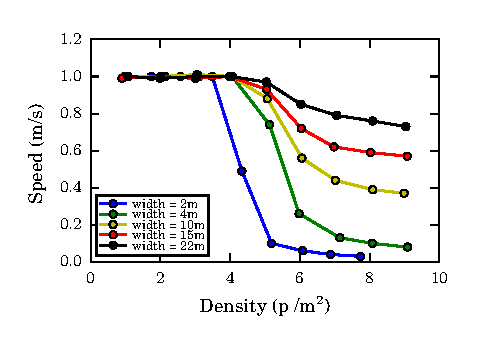
\includegraphics[width=\columnwidth]
{plots/speed-density_vd1_multiple_widths.eps}
\caption{\label{fig:2} Speed as a function of the density for different widths. Inittialy, 
pedestrians were random distributed along the corridor. The measurements were taken in the middle
of the corridor once the system reached the stationary state. The lenght of the corridor 
was 28~m in all cases with periodic boundary conditions in the x direction.}
\end{figure}


\begin{comment}
\subsection{\label{evacuation}Evacuation time versus the desired velocity}

\begin{equation}
v^{-1}\sim \displaystyle\frac{\ln(\beta 
v_d/A)}{\beta v_d/A}\label{constrain2}
\end{equation}

\end{comment}
